\documentclass[spanish]{udpreport}
\usepackage[utf8]{inputenc}
\usepackage[spanish]{babel}

% Podemos establecer el logo de alguna entidad o dejar el de la UDP (defecto)
%\setlogo{EITFI}

\title{Informe de redes de datos 1\\
"Cableado Estructurado"\\}
\author{Alumno: Camilo Araya
\\Profesor: Nicolás Hidalgo\\Ayudante: Martín Griño}
\date{30 de agosto de 2017}

% Además podemos establecer la facultad y escuela
% los valores por defecto son los siguientes:
%\udpschool{Escuela de Informática y Telecomunicaciones}
%\udpfaculty{Facultad de Ingeniería}
%\udpuniversity{Universidad Diego Portales}

\begin{document}
\maketitle

\chapter*{Resumen} 
\addcontentsline{toc}{section}{Resumen} 
\markboth{RESUMEN}{RESUMEN} 

El presente informe tiene por objetivo observar, analizar y construir un cable de conexión entre redes, ya sea de iguales tipos de dispositivos como también distintos, los cuales mediante la practica junto con la teoría establecida del cable de red los cuales serán fundamentales para comprender en profundidad el tópico. 
\\ 
\\
En esta experiencia se abordara la construcción de dos cables de red (Directo y Cruzado) orientándose por la norma EIA/TIA-568B.






\tableofcontents

\chapter{Introducción}
Los conocimientos básicos del cableado estructurado al momento de montar una red de datos computacionales son de suma importancia para definir una variedad de conceptos elementales que son la base en la actualidad en lo que a el mundo de la informática y de las telecomunicaciones se refiere, junto con esto también se abordaran las aplicaciones, sus normas y datos que pueden ser relevantes con respecto al cableado estructurado.


\section{Usos del cableado estructurado}

\subsection{Área de trabajo}
Lugar que concentra a los operadores de dispositivos computacionales de variados tipos(computadores, impresoras,teléfonos,smartphones,etc),donde la norma indica que el cableado del panel de cada área de trabajo debe conectarse de forma horizontal.
\subsection{Cuarto de telecomunicaciones}
Los cuartos de telecomunicaciones se les conoce generalmente como IDF (Intermediate Distribution Facility), estos generalmente corresponden a cuartos que conectan todo el cableado horizontal correspondiente al área de trabajo en cuestión. Los MDF (Main Distribution Facility) corresponde al nodo que interconecta a todos los IDF's que se encuentran en las distintas plantas de un edificio, este tipo de instalaciones los cableados se conectan de forma vertical.
\subsection{Punto de acceso a internet}
También conocido como POP (point of Presence) lugar donde se conecta el MDF del edificio con la red de internet ISP de telecomunicaciones.
\section{Normas de cableado estructurado}
Los cableados estructurados están normalizados por estándares internacionales que regulan todas las instalaciones,son de vital importancia dado que regulan los flujos de datos entre distintos dispositivos y redes.
\subsection{Configuración EIA/TIA 568(A/B)}
Esta configuración permitirá la creación de  un cable de red normalizado, de estas se pueden distinguir las conexiones directas y cruzadas.
En cuanto al cable mas utilizado en este tipo redes es cable de cobre cat5 el cual garantiza las comunicaciones con un gran ancho de banda.
\chapter{Marco teórico}
\section{Indicaciones técnicas}
\subsection{Cable UTP}
El cable a utilizar en la experiencia es un cable UTP cat5, correspondiente a un cable de bajo costo,trenzado no blindado. Este cable se encuentra estandarizado bajo la normas EIA/TIA 568B y ISO/IEC 11801.
\begin{figure}[h]
    \centering
    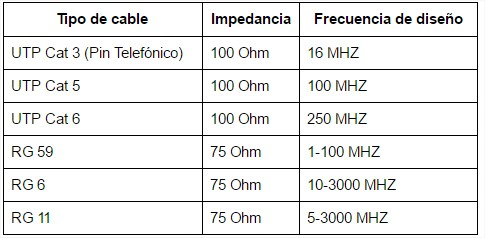
\includegraphics[scale=0.3]{images/FrecuenciaCable.jpg}
    \caption{Cables UTP y sus caracteristicas}
    \label{fig:my_label}
\end{figure}
\subsection{Cabezal RJ-45}
Corresponden a conectores hembra donde se conecta el cableado UTP,este tiene 8 pines que conectan la electricidad desde una fuente hacia el cable y logrando de esa forma transferir paquetes de datos hacia varios destinatarios.

\subsection{Crimpeadora RJ-45}
Es una indispensable herramienta para la construcción de cables de red, esta permite cortar y crimpear cables UTP, también permite instalar los conectores Rj-45.
\newpage
\section{Conexiones}
El cableado estructurado tiene variados usos en el ámbito de redes de datos, este suele conectar dispositivos de iguales características o distintas logrando que el flujo de información fluya en la dirección que nosotros queramos.
Existen dos tipos de conexiones en función de los dispositivos que queramos utilizar, esta es la conexión directa (straight through) y la conexión cruzada (crossover).

\begin{figure}[h]
    \centering
    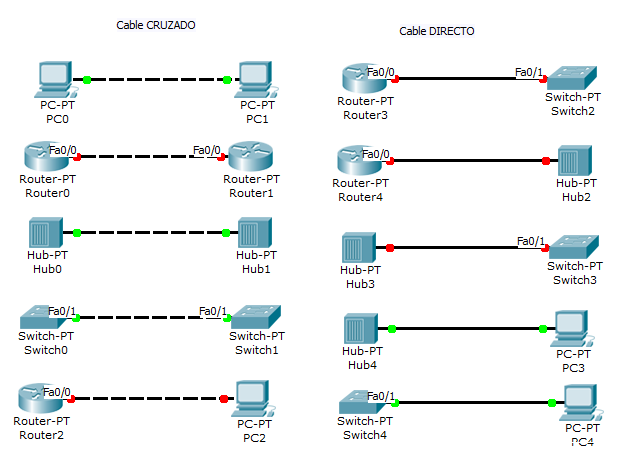
\includegraphics{images/tipos-cables-conexion.png}
    \caption{Imagen de conexiones}
    \label{fig:my_label}
\end{figure}

\chapter{Marco practico}
\section{Primer paso}
Se nos hizo la entrega de un cable cat5, tres conectores RJ-45 y una crimpeadora. Luego se realizo una breve introducción de como construir nuestro cable de red y de que forma utilizar las herramientas entregadas.
\begin{figure}[h]
    \centering
    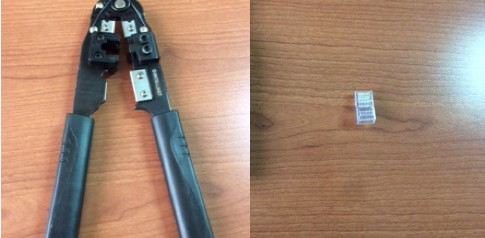
\includegraphics[scale=0.3]{images/1.jpg}
    \caption{Crimpeadora y cabezal Rj-45}
    \label{fig:my_label}
\end{figure}
\section{Segundo paso}
Se procedió a realizar la conexión directa, para ello crimpeamos ambos extremos del cable, En ambos extremos cortamos en aproximadamente 0.7 cm la capa superficial dejando a la vista los cables internos los cuales estaban representado por colores. Luego de ubicar y ordenar los cables con la configuración EIA/TIA 568B montamos el cabezal RJ-45 generando el cable de red directo.
\begin{figure}[h]
    \centering
    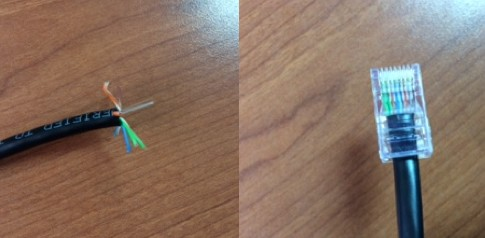
\includegraphics[scale=0.2]{images/2.jpg}
    \caption{Corte del cable y unión con cabezal RJ-45}
    \label{fig:my_label}
\end{figure}
\\
La conexión directa es usada generalmente para conectar  distintos dispositivos, en ambos extremos del cable deben presentar la misma distribución, como se muestra en la siguiente imagen" Representación 1".
\begin{figure}[h]
    \centering
    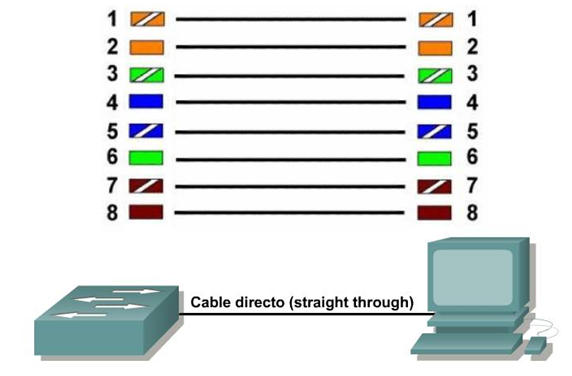
\includegraphics[scale=0.2]{images/direc.png}
    \caption{Representación 1 }
    \label{fig:my_label}
\end{figure}
\newpage
\section{Tercer paso}
Luego de montar el cable directo y comprobar a través de un tester si efectivamente cumplía con los estándares se procedió a cortar nuevamente el cable y en uno de sus extremos se volvió a conectar un cabezal RJ-45, pero con la configuración y unión de sus cables según la norma EIA/TIA 568A, como se muestra el la siguiente imagen "Representación 2".\\
\begin{figure}[h]
    \centering
    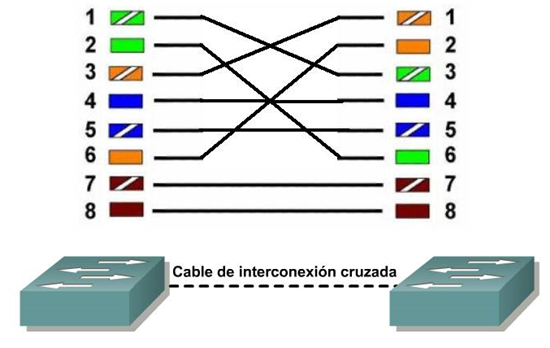
\includegraphics[scale=0.3]{images/cruzad.png}
    \caption{Representación 2}
    \label{fig:my_label}
\end{figure}
\\
Luego de ubicar y ordenar los cables se monta nuevamente el cabezal generando nuestro cable de red cruzado como se muestra el la siguiente imagen(Cable de red Cruzado):
\\
\begin{figure}[h]
    \centering
    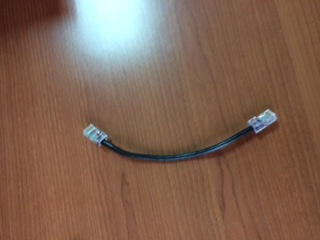
\includegraphics{images/image1.jpeg}
    \caption{Cable de red cruzado}
    \label{fig:my_label}
\end{figure}
\newpage
\chapter{Conclusión}
A partir de lo realizado en la experiencia de laboratorio se destaca que para la elaboración de un cable de  red, se tienen que tener en consideración algunos conceptos  y reglas básicas que permitirán una correcta implementación al momento de poner en práctica su construcción, es decir, como punto de partida se tiene que tener claro que tipo de cable se requiere construir dependiendo de que uso quiera darse (directo o cruzado), por otro lado se especifica que en todo momento se siguió la norma ANSI/TIA/EIA 568B la cual tiene dos configuraciones de conexión que son T568A y T568B.\\
Para la construcción del cable directo durante la experiencia se usó la norma con la configuración T568B en ambos extremos, posteriormente, para la construcción del cable cruzado se procede a cortar uno de los extremos del cable para cambiarla por una nueva configuración T658A, logrando así los objetivos principales de la práctica de laboratorio.\\
Bajo el concepto mencionado anteriormente y con lo puesto en práctica en la experiencia se logra comprender de manera satisfactoria las diferencias del cable directo y cruzado, también se logra entender que norma y configuraciones deben cumplirse para lograr que la construcción del cable sea exitosa en el ámbito que desee implementarse, por ejemplo si conecto un computador y un Hub la conexión será directa, por otro lado, si quiero conectar dos computadores entre sí, la conexión tendrá que ser cruzada.
\begin{thebibliography}{0}
\bibitem{1}Características conectores RJ-45. Recuperado de http://www.ds3comunicaciones.com/satra/SA-300102-6.html
\bibitem{2}Usos de la red. Recuperado de https://www.ecured.cu/Red-de-computadoras

\end{thebibliography}
\listoffigures
\end{document}

